\begin{figure*}[t]
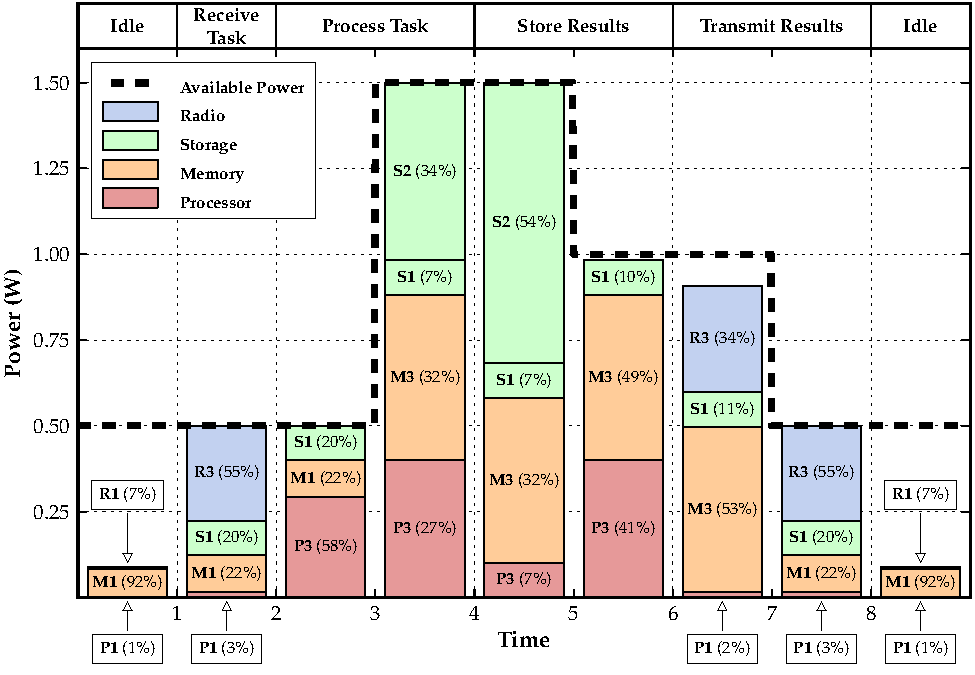
\includegraphics[width=\textwidth]{./figures/transitiongraph.pdf}
\noindent\begin{minipage}[t]{0.5\textwidth}
\vspace{-0.05in}
\begin{tabularx}{\columnwidth}{cX}

\textbf{0} & When idle \textbf{P1} and \textbf{M1} are idled and \textbf{R1}
operates at low duty cycle.
\\

\textbf{1} & Receiving data over \textbf{R1} the phone initiates a background
task. The device activates \textbf{R2} to rapidly receive data and
\textbf{S1} to store it.
\\

\textbf{2} &
As the phone begins processing the task it activates \textbf{P2} and disables
\textbf{R2}.
\\

\textbf{3} &
The user removes the phone from their pocket and begins interacting with an
application, which activates \textbf{M2} and retrieves data from \textbf{S2}.
\\

\end{tabularx}

\end{minipage}
\begin{minipage}[t]{0.5\textwidth}
\vspace{-0.05in}

\begin{tabularx}{\columnwidth}{cX}

\textbf{4} & As the interactive application continues energy usage shifts
from \textbf{S2} to \textbf{P2}.
\\

\textbf{5} & When the interactive application is finished with \textbf{S2} it
is disabled.
\\

\textbf{6} & As the interactive session completes, the phone offloads data
using \textbf{R2} driven by \textbf{P1}.
\\

\textbf{7} & Background processing resumes in the same ensemble it was using
previously.
\\

\textbf{8} &
The background task completes, idling the phone.
\\

\end{tabularx}
\end{minipage}
\vspace{-0.1in}
\caption{\normalsize \textbf{Scenario.} The figure and table describe the
scenario referred to throughout Section~\ref{sec-challenges}. Bars indicate
the total energy consumed, broken down and labeled by component. The table
describes what is happening at each time step.}

\label{figure-transitiongraph}
\vspace{0.10in}
\hrule
\vspace{-0.20in}
\end{figure*}
